% ================================================
% =                 EXPERIMENTS                  = 
% ================================================ 

This section includes all experiments carried out for evaluating the difference between the two approaches considered in the BEV2Seg\_2 pipeline, experiments to study what is the influence of extrinsic parameters modification as data augmentation technique for semantic segmentation of BEV images and the final evaluation of the proposed annotation pipeline of occupancy, occlusion and driveable areas.

\subsection{BEV2Seg\_2}
Both approaches, segmenting-then-IPM and IPM-then-segmenting, were trained under the same conditions: the encoder layers were not frozen during fine-tuning for the segmentation task, allowing the entire model to adapt to the data. Input image preprocessing was performed using the \textit{SegformerImageProcessor}, which includes resizing the images to $512 \times 512$ pixels, rescaling pixel values by a factor of $1/255$, and normalizing using the mean and standard deviation values from ImageNet~\cite{imagenet}. This ensures the input format is consistent with what the pretrained encoders expect.

Additionally, during training, semantic masks were provided with the \texttt{reduce\_labels} parameter set to \texttt{False}, since our dataset includes the "background" class. This means gradients are computed for all image regions during training. All experiments were carried out using the same hardware configuration described in Table~\ref{tab:hardware}. Among the six available Segformer encoder variants, three were selected for evaluation: MiT-b0, MiT-b2, and MiT-b4.

\hl{Complete this table.}
\begin{table}[h]
    \centering
    \begin{tabular}{c l c}
        \toprule
        \textbf{Component} & \textbf{Specifications} & \textbf{Num workers} \\
        \midrule
        CPU         & - & 8 \\
        GPU         & - & 2 \\      
        Memmory     & - & - \\
        OS          & - & - \\
        \bottomrule
    \end{tabular}
    \caption{ Hardware used for experiments }
    \label{tab:hardware}
\end{table}

Regarding to the used notation, the models that follow the segment-then-IPM pipeline to obtain BEV semantic masks are referred to as \texttt{raw2seg\_bev}, while those that first apply IPM and then perform segmentation are named \texttt{raw2bev\_seg}.

The two approaches were firstly trained using the smallest Segformer model variant, MiT-b0, for $20.7K$ steps without applying any regularization techniques. This initial experiment was carried out to observe whether the models were able to learn and predict on the dataset and see if them suffered from overfitting. Also, for this purpose, the choice of MiT-b0 was intentional as it trains faster and, due to its limited capacity, is less prone to extreme overfitting compared to larger models. This made it a suitable candidate for testing different hyperparameter configurations in a lightweight environment.

\hl{I didn't find what is the segformer's loss function.}

As shown in Figure~\ref{fig:overfitting_mit-b0}, both models showed clear signs of overfitting. While the training loss continued to decrease continuously, the validation loss began to increase, indicating a lack of generalization and failure to converge. These results highlight the importance of introducing regularization techniques even for small model sizes. Additionally, no signs of exploding gradients were observed during the training of these models.

\begin{figure}[h!]
    \centering
    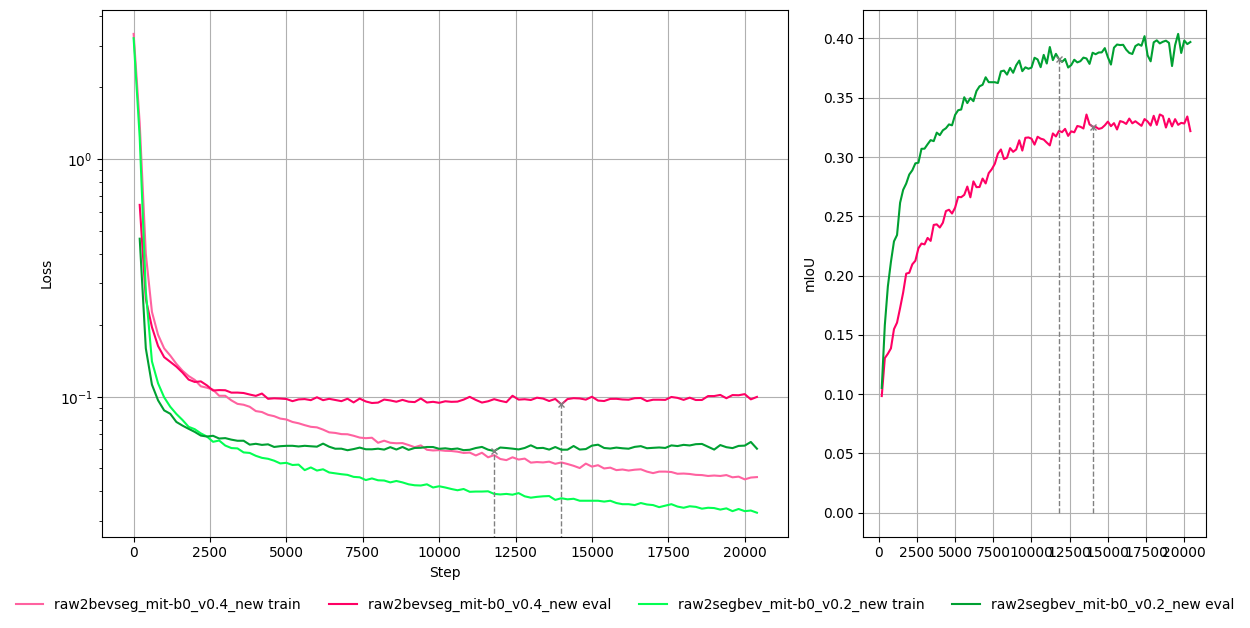
\includegraphics[width=0.7\linewidth]{./images/experiments/overfitting_bev_nu.png}
    \caption{Training and evaluation loss of raw2seg\_bev and raw2bev\_seg MiT-b0 models without any regularization technique}
    \label{fig:overfitting_mit-b0}
\end{figure}

It is important to note that the evaluation datasets differ between the two pipelines as one evaluates performance on BEV projections while the other does so on regular images motivating the gap in their validation results.

To address the overfitting, data augmentation strategies described in Section~\ref{sec:data_augmentations} were applied to introduce variability in the training data. Additionally, other regularization methods such as weight decay (also known as L2 regularization) were employed. Weight decay penalizes large weights during training, and makes the model more robust and less prone to memorizing irrelevant details. With these regularization techniques in place, the overfitting behavior was significantly reduced as shown in Figure~\ref{fig:before_after_data_aug}.

\hl{Temporal graph!!}
\begin{figure}[h!]
    \centering
    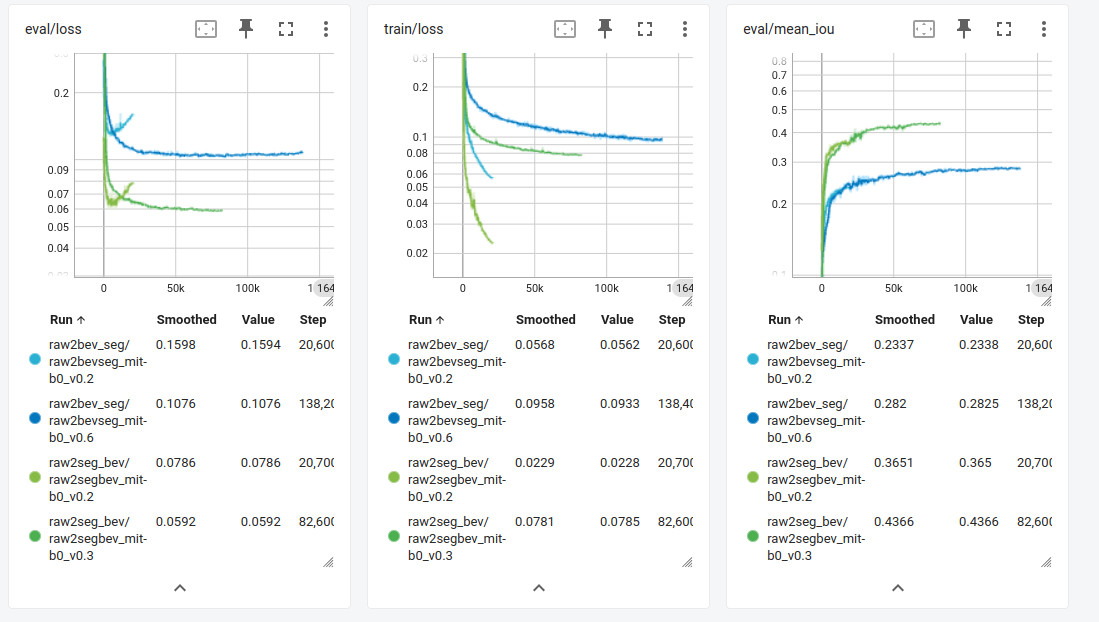
\includegraphics[width=0.7\linewidth]{./images/experiments/before_an_after_data_aug.png}
    \caption{Before and after regularization techniques. Light colors before, darker colors after. BEV segmentation model uses normal data augmentations.}
    \label{fig:before_after_data_aug}
\end{figure}

\hl{Comment that with model size MiT-b4 gradient accumulation techniques were used to fit the GPU memory specs.}

\hl{Comment the max epochs set to 200 and the checkpoint strategy used: it is controvesial wheter to use the loss or mIoU. Whe have decided to use the loss.}

With all of this in place, the training strategy is designed to support experimentation in order to answer two main research questions: In the case of segmentation in BEV images, \textit{which data augmentation technique is more effective: using the same strategy applied in the other approach, or modifying the extrinsic camera parameters?}; and \textit{which of the two approaches performs better for BEV image segmentation?}

\subsubsection{BEV images data augmentation techniques comparison}
\hl{Comparison between normal geometric data augmentation techniques and camera's extrinsic parameters modifications.}


\subsubsection{Pipeline comparison}
\hl{raw2seg\_bev results compared with raw2bev\_seg results.}

\subsection{3D detections evaluations}
\hl{Explain the selected NuScenes selected vehicle scene, and expose the metrics used (mIoU and v2v distance).}

\subsection{BEV masks evaluation}
\hl{Groundtruth BEV masks could be generated from annotations and compute mIoU between the annotated BEV masks and ground truth ones.}

